\documentclass[border=4pt]{standalone}
\usepackage[T1]{fontenc}
\usepackage{lmodern}
\usepackage{amsmath}
\usepackage{tikz}
\usetikzlibrary{positioning,arrows.meta,calc}
\begin{document}
\sffamily\footnotesize
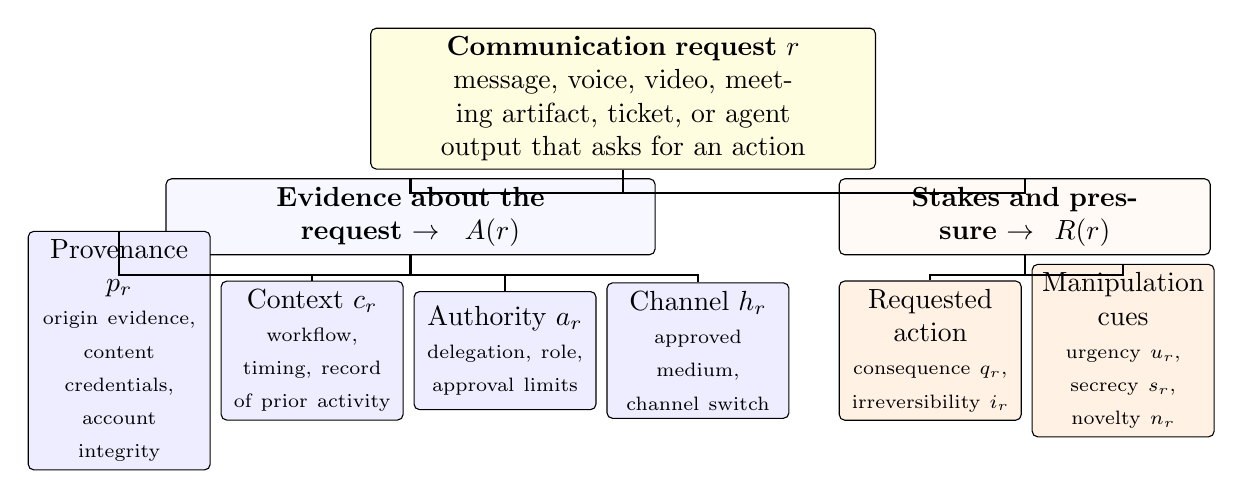
\begin{tikzpicture}[
  box/.style={draw, rounded corners=2pt, align=center, minimum height=8mm, inner sep=3pt},
  ev/.style={box, fill=blue!7, text width=21mm, minimum height=15mm},
  pr/.style={box, fill=orange!10, text width=21mm, minimum height=15mm},
  ln/.style={thick}
]
\node[box, fill=yellow!12, text width=62mm] (r) at (6.4,3.2) {\textbf{Communication request $r$}\\ message, voice, video, meeting artifact, ticket, or agent output that asks for an action};
\node[box, fill=blue!3, text width=60mm] (E) at (3.7,1.7) {\textbf{Evidence about the request} $\rightarrow A(r)$};
\node[box, fill=orange!4, text width=45mm] (P) at (11.5,1.7) {\textbf{Stakes and pressure} $\rightarrow R(r)$};
\node[ev] (p) at (0,0) {Provenance $p_r$\\{\scriptsize origin evidence, content credentials, account integrity}};
\node[ev] (c) at (2.45,0) {Context $c_r$\\{\scriptsize workflow, timing, record of prior activity}};
\node[ev] (a) at (4.9,0) {Authority $a_r$\\{\scriptsize delegation, role, approval limits}};
\node[ev] (h) at (7.35,0) {Channel $h_r$\\{\scriptsize approved medium, channel switch}};
\node[pr] (act) at (10.3,0) {Requested action\\{\scriptsize consequence $q_r$, irreversibility $i_r$}};
\node[pr] (cue) at (12.75,0) {Manipulation cues\\{\scriptsize urgency $u_r$, secrecy $s_r$, novelty $n_r$}};
\draw[ln] (r.south) -- ++(0,-0.3) -| (E.north);
\draw[ln] (r.south) -- ++(0,-0.3) -| (P.north);
\foreach \n in {p,c,a,h} \draw[ln] (E.south) -- ++(0,-0.25) -| (\n.north);
\foreach \n in {act,cue} \draw[ln] (P.south) -- ++(0,-0.25) -| (\n.north);
\end{tikzpicture}
\end{document}
